\chapter{Applications of de Rham Cohomology}
Let us introduce the standard notation\index{$n$-ball}\index{$n$-sphere}
\begin{align*}
  & D^n = \{x \in \RR^n \mid \| x \| \leq 1\} && \text{ the $n$-ball } \\
  & S^{n-1} = \{x \in \RR^n \mid \| x \| = 1\} && \text{ the $(n-1)$-sphere } 
\end{align*}

A fixed point for a map $f:x\to X$ is a point $x\in X$, such that $f(x) = x$.

\begin{theorem}[Brouwer's fixed point theorem, 1912]\label{theorem:7-1}
  Every continuous map $f:D^n \to D^n$ has a fixed point.
\end{theorem}

\begin{proof}
  Assume that $f(x)\neq x$ for all $x\in D^n$. For every $x\in D^n$ we can define 
  the point $g(x)\in S^{n-1}$ as the point of the intersection between $S^{n-1}$ ans the half-line 
  from $f(x)$ to $x$.

\begin{figure}[!htb]
  \centering
  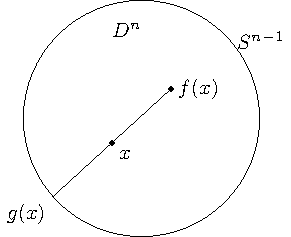
\includegraphics[width=.3\linewidth]{./pics/page-47.pdf} 
  % \caption{}
  \label{fig:page-47}
\end{figure}

We have that $g(x) = x+tu$, where $u=\frac{x-f(x)}{\|x-f(x)\|}$, and 
\begin{align*}
  t = -x\cdot u + \sqrt{1-\|x\|^2 + (x\cdot u)^2}
\end{align*}

Here $x\cdot u$ denotes the usual inner product. The expression for $g(x)$ is obtained
by solving the equation $(x + tu)\cdot(x + tu) = 1$. There are two solutions since the
line determined by $f(x)$ and $x$ intersects $S^{n-1}$ in two points. We are interested in
the solution with $t\ge 0$. Since $g$ is continuous with $g|_{S^{n-l}} = \id_{S^{n-l}}$, the 
theorem follows from the lemma below.
\end{proof}

\begin{lemma}\label{lemma:7-2}
  There is no continuous map $g:D^n\to S^{n-1}$, with $g|_{S^{n-l}} = \id_{S^{n-l}}$.
\end{lemma}

\begin{proof}
  We may assume that $n\ge 2$. For the map $r:\RR-\{0\}\to \RR^n-\{0\}, r(x)=x/\|x\|$, we 
  get that $\id_{\RR^n-\{0\}}\sime r$, because $\RR^n-\{0\}$ always contains the line
  segment between $x$ and $r(x)$ (see Example \ref{example:6-5}). If $g$ is of the indicated 
  type, then $g(t\cdot r(x)), 0\le t\le 1$ defines a homotopy from a constant map to $r$. This 
  shows that $\RR^n-{0}$ is contractible. Corollary \ref{corollary:6-10} asserts that $H^{n-1}(\RR^n-\{0\}) = 0$,
  which contradicts Theorem \ref{theorem:6-13}
\end{proof}

The tangent space of $S^n$ in the point $x\in S^n$ is $T_xS^n = \{x\}^\perp$, the orthogonal
complement in $\RR^{n+1}$ to the position vector. A tangent vector field on $S^n$ is a continuous
map $v:S^n\to\RR^{n+1}$ such that $v(x)\in T_xS^n$ for every $x\in S^n$.

\begin{theorem}\label{theorem:7-3}
  The sphere $S^n$ has a tangent vector field $v$ with $v(x)\neq 0$ for all $x\in S^n$ if and 
  only if $n$ is odd.
\end{theorem}

\begin{proof}
  Such a vector field $v$ can be extended to a vector field $w$ on $\RR^n-\{0\}$
  by setting
  \begin{align*}
    w(x) = v(\frac{x }{\|x\|})
  \end{align*}

  We have that $w(x)\neq 0$ and $w(x)\cdot x = 0$. The expression 
  \begin{align*}
    F(x, t) = (\cos\pi t)x + (\sin\pi t)w(x)
  \end{align*}

  defines a homotopy from $f_0=\id_{\RR^{n+1}-\{0\}}$ to the antipodal map $f_1,f_1(x)=-x$.
  Theorem \ref{theorem:6-8}.(i) shows that $f_i^*$ is the identity on $H^n{\RR^{n+1}-\{0\}}$, which by
  Theorem \ref{theorem:6-13} is 1-dimensional. On the other hand Lemma 6.14 evaluates $f_i^*$ to
  be multiplication with $(-1)^{n+1}$. Hence $n$ is odd.
  Conversely, for $n=2m-1$, we can define a vector field $v$ with 
  \begin{align*}
    v(x_1,x_2,\cdots,x_{2m}) = (-x_2, x_1, -x_4, x_3, \cdots, -x_{2m}, x_{2m-1}).
  \end{align*}
\end{proof}

In 1962 J. F. Adams solved the so-called "vector field problem": find the maximal
number of linearly independent tangent vector fields one may have on $S^n$.
(Tangent vector fields $v_1,\cdots,v_d$ on $S^n$ are called linearly independent if for every
$s\in S^n$ the vectors $v_1(x),\cdots,v_d(x)$ are linearly independent.)

\paragraph{\textbf{Adams' theorem}\label{adams-theorem}
  For $n=2m-1$, let $2m=(2c+1)2^{4a+b}$, where $0\le b\le 3$. The maximal number of linearly independent 
  tangent vector field on $S^n$ is equal to $2^b+8a-1$.
}

\begin{lemma}[Urysohn-Tietze]\label{lemma:7-4}\index{Urysohn-Tietze lemma}
  If $A\subseteq \RR^n$ is closed and $f:A\to\RR^n$ continuous, then there exists a continuous map 
  $g:\RR^n\to\RR^m$ with $g|_A = f$.
\end{lemma}

\begin{proof}
  We denote Euclidean distance in $\RR^n$ by $d(x, y)$ and for $x\in\RR^n$ we define 
  \begin{align*}
    d(x, A) = \inf_{y\in A} d(x, y)
  \end{align*}
  For $p\in\RR^n-A$ we have an open neighborhood $U_p\subseteq\RR^n-A$ of $p$ given by 
  \begin{align*}
    U_p = \left\{x\in\RR^n\big| d(x, p)< \frac12d(p, A)\right\}
  \end{align*}
  These sets cover $\RR^n-A$ and we can use Theorem \ref{theorem:A.1} to find a subordinate
  partition of unity $\phi_p$. We have $g$ by 
  \begin{align*}
    g(x) = \left\{\begin{aligned}
      & f(x) && \text{ if } x\in A \\
      & \sum_{p\in\RR^n-A}\phi_p(x)f(a(p)) && \text{ if } x\in\RR^n-A
    \end{aligned}\right.
  \end{align*}

  where $p\in\RR^n - A, a(p)\in A$ is chosen such that 
  \begin{align*}
    d(p, a(p))< 2d(p, A)
  \end{align*}
  Since the sum is locally finite on $\RR^n-A$, $g$ is smooth on $\RR^n-A$
  The only remaining problem is the continuity of $g$ at a point $x_0$ on the boundary
  of $A$. If$ x\in U_p$ then
  \begin{align*}
    d(x_0, p) 
      \le d(x_0, x) + d(x, p)
      < d(x_0, x) + \frac12d(p, A)
      \le d(x_0, x) + \frac12d(p, x_0).
  \end{align*}
  Hence $d(x_0, p)<2d(x_0, x)$ for $x\in U_p$. Since $d(p, a(p))<2d(p, A)\le d(x_0, p)$, we get 
  for $x\in U_p$ that $d(x_0, a(p))\le d(x_0, p) + d(p, a(p))<3d(x_0, p)<6d(x_0, x)$. For $x\in\RR^n-A$
  we have 
  \begin{align*}
    g(x) - g(x_0)
    = \sum_{p\in\RR^n-A}^{}{\phi_p(x)(f(a(p)) - f(x_0))}
  \end{align*}
  and 
  \begin{align}\label{eq:7-1}
    \|g(x)-g(x_0)\| \le \sum_{p}^{}{\phi_p(x) \|f(a(p)) - f(x_0)\|},
  \end{align}
  where we sum over the points $p$ with $x\in U_p$. 
  For an arbitary $\epsilon>0$ choose $\delta >0$ such that $\|f(y)-f(x_0)\|<\epsilon$ for every 
  $y\in A$ with $d(x_0, y)<6\delta$. If $x\in\RR^n-A$ and $d(x, x_0)<\delta$ then, for $p$ with 
  $x\in U_p$, we have that $d(x_0, a(p))<6\delta$ and $\|f(a(p)) - f(x_0)\|<\epsilon$. Then 
  \eqref{eq:7-1} yields
  \begin{align*}
    \|g(x) - g(x_0)\| \le \sum_{p}^{}{\phi_p(x)\cdot\epsilon} = \epsilon.
  \end{align*}
  Continuity of $g$ at $x_0$ follows.
\end{proof}

\begin{remark}\label{remark:7-5}
  The proof above still holds, with marginal changes, when $\RR^n$ is
  replaced by a metric space and $\RR^m$ by a locally convex topological vector space.
\end{remark}

\begin{lemma}\label{lemma:7-6}
  Let $A\subseteq\RR^n$ and $B\subseteq\RR^m$ be closed sets and let $\phi:A\to B$ be a 
  homeomorphism. There is a homeomorphism $h$ of $\RR^{n+m}$ to itself, such that 
  \begin{align*}
    h(x, 0_m) = (0_m, \phi(x))
  \end{align*}
  for all $x\in A$.
\end{lemma}

\begin{proof}
  By Lemma \ref{lemma:7-4} we can extend $\phi$ to a continuous map $f_1:\RR^n\to\RR^m$. A 
  homeomorphism $h_1:\RR^n\times\RR^m\to\RR^n\times\RR^m$ is defined by 
  \begin{align*}
    h_1(x, y) = (x, y+f_1(x)).
  \end{align*} 
  The inverse to $h_1$ is obtained by subtracting $f_1(x)$ instead. Analogously we can 
  extend $\phi^{-1}$ to a continuous map $f_2:\RR^m\to\RR^n$ and defines a homeomorphism
  $h_2:\RR^n\times\RR^m$ by 
  \begin{align*}
    h_2(x, y) = (x+f_2(y), y).
  \end{align*}
  If $h$ is defined to be $h=h_2^{-1}\circ h_1$, then we have for $x\in A$ that 
  \begin{align*}
    h_1(x, 0_m) 
    = h_2^{-1}(x, f_1(x))
    = h_2^{-1}(x, \phi(x))
    = (x-f_2(\phi(x)), \phi(x))
    = (0_n,  \phi(x)).
  \end{align*}
\end{proof}

We identity $\RR^n$ with the subspace of $\RR^{n+m}$ consisting of vectors of the form 
\[(x_1, \cdots, x_n, 0, \cdots, 0).\]

\begin{corollary}\label{corollary:7-7}
  If $\phi:A\to B$ is a homeomorphism between closed subsets $A$ and $B$
  of $\RR^n$, then $\phi$ can be extended to a homeomorphism $\phi:\RR^{2n}\to\RR^{2n}$.
\end{corollary}

\begin{proof}
  We merely have to compose the homeomorphism h from Lemma 7.6 with
the homeomorphism of $\RR^{2n} = \RR^{2n}\times\RR^{2n}$ to itself that switches the two 
factors.
\end{proof}

Note that $\phi$ by restriction gives a homeomorphism between $\RR^{2n}-A$ and $\RR^{2n}-B$.
In contrast it can occurs that $\RR^n-A$ is not homeomorphism to $\RR^n-B$. A well-known example 
is \Index{Alexander's ``horned sphere''} $\Sigma$ in $\RR^3$: $\Sigma$ is homeomorphism to $S^2$, but 
$\RR^30\Sigma$ is not homeomorphism to $\RR^3-S^2$. This and numerous examples are treated in [Rushing].


\begin{theorem}\label{theorem:7-8}
  Assume that $A\neq\RR^n$ and $B\neq\RR^n$ are closed subsets of $\RR^n$. If $A$ and $B$
  are homeomorphism, then 
  \begin{align*}
    H^p(\RR^n-A)\simee H^p(\RR^n-B)
  \end{align*}
\end{theorem}

\begin{proof}
  By induction on $m$ Proposition \ref{prop:6-11} yields isomorphism 
  \begin{align*}
    & H^{p+m}(\RR^{n+m}-A)\simee H^p(\RR^n-A) \\
    & H^{m}(\RR^{n+m}-A)\simee H^0(\RR^n-A)/\RR\cdot 1 
  \end{align*}
  for all $m\ge 1$. Analogously for $B$. From Corollary \ref{corollary:7-7} we known that $\RR^n-A$
  and $\RR^{2n}-B$ are homeomorphic. Topological invariance (Corollary \ref{corollary:6-9}) shows that 
  they are isomorphic de Rham cohomologies. We thus have the isomorphism
  \begin{align*}
    H^p(\RR^n-A) 
      \simee H^{p+n}(\RR^{2n}-A) 
      \simee H^{p+n}(\RR^{2n}-B)
      \simee H^p(\RR^n-B)
  \end{align*}
  for $p>0$ and 
  \begin{align*}
    H^p(\RR^n-A)/\RR\cdot 1
      \simee H^{p+n}(\RR^{2n}-A) 
      \simee H^{p+n}(\RR^{2n}-B)
      \simee H^p(\RR^n-B)/\RR\cdot 1
  \end{align*}
\end{proof}

For a closed set $A\subseteq\RR^n$ the open complement $U=\RR^n-A$ will always be
a disjoint union of at most countably many connected components, which all
are open. If there are infinitely many, then $H^0(U)$ will have infinite dimension.
Otherwise the number of connected components is equal to dim $H^0(U)$.


\begin{corollary}\label{corollary:7-9}
  If $A$ and $B$ are two homeomorphic closed subsets of $\RR^n$, then $\RR^n-A$
and $\RR^n- B$ have the same number of connected components.
\end{corollary}


\begin{proof}
  If $A\neq \RR^n$ and $B\neq \RR^n$ the assertion follows from Theorem \ref{theorem:7-8} and 
  the remarks above. If $A= \RR^n$ and $B\neq \RR^n$ then $\RR^{n+1}-A$ has precisely 2 connected
  components (the open half-spaces), while $\RR^{n+l} - B$ is connected. Hence this case 
  cannot occur.
\end{proof}


\begin{theorem}[Jordan-Brouwer separation theorem]\label{theorem:7-10}
\index{Brouwer theorem}\index{Jordan-Brouwer theorem}
  If $\Sigma\subseteq\RR^n, (n\ge 2)$ is homeomorphic to $S^{n-1}$ then 
  \begin{enumerate}[(i)]
    \item $\RR^n-\Sigma$ has precisely 2 connected components $U_1$ and $U_2$, where 
      $U_1$ is bounded and $U_2$ is unbounded.
    \item $\Sigma$ is the set of boundary points for both $U_1$ and $U_2$.
  \end{enumerate}
  We say $U_1$ is the domain inside $\Sigma$ and $U_2$ the domain outside $\Sigma$.
\end{theorem}

\begin{proof}
  Since $\Sigma$ is compact, $\Sigma$ is closed in $\RR^n$. To show (i), it suffices, by Corollary
  \ref{corollary:7-9}, to verify it for $S^{n-1}\subseteq\RR^n$. The two connected components of $\RR^n-S^{n-1}$
  are 
  \begin{align*}
    D^n = \{x\in \RR^n\big|\|x\|<1 \} \text{ and } W = \{x\in\RR^n\big| \|x\|>1\}
  \end{align*}
  By choosing $r=\max\limits_{x\in\Sigma}\|x\|$, the connected set 
  \begin{align*}
    rW = \{x\in\RR^n \big| \|x\|>r\}
  \end{align*}
  will be contained in one of the two components in $\RR^n-\Sigma$, and the other component
must be bounded. This completes the proof of (i).

  Let $p\in\Sigma$ be given and consider an open neighbourhood $V$ of $P$ in $\RR^n$. The set
  $A=\Sigma-(\Sigma\cap V)$ is closed and homeomorphic to a corresponding proper closed
  subset $B$ of $S^{n-1}$. It is obvious that $\RR^n-B$ is connected, so by Corollary \ref{corollary:7-9}
  the same is the case for $\RR^n-A$. For $p_1\in U_1$ and $p_2\in U_2$, we can find a continuous curve 
  $\gamma:[a, b]\to\RR^n-A$ with $\gamma(a)=p_1$ and $\gamma(b)=p_2$. By (i) the curve must intersect 
  $\Sigma$, i.e. $\gamma^{-1}(\Sigma)$ is nonempty. The closed set $\gamma^{-1}(\Sigma)\subseteq[a, b]$ has 
  a first element $c_1$ and a last element $c_2$, which both belong to $(a, b)$. Hence $\gamma(c_1)\in\Sigma\cap V$
  and $\gamma(c_2)\in\Sigma\cap V$ are points of contact for $\gamma([a, c_1))\subseteq U_1$ and 
  $\gamma([a, c_2))\subseteq U_2$ respectively. Therefore we can find $t_1\in [a, c_1)$ and $t_2\in[c_2, b)$,
  such that $\gamma(t_1)\in U_1\cap V$ and $\gamma(t_2)\in U_2\cap V$. This shows that $p$ is a boundary
  point for both $U_1$ and $U_2$, and proves (ii).
\end{proof}

\begin{theorem}\label{theorem:7-11}
  If $A\subseteq\RR^n$ is homeomorphic to $D^k$, with $k\le n $, then $\RR^n-A$ is connected.
\end{theorem}

\begin{proof}
  Since $A$ is compact, $A$ is closed. By Corollary \ref{corollary:7-9} it is sufficient to prove
the assertion for $D^k\subseteq\RR^k\subseteq\RR^n$. This is left to the reader.
\end{proof}

\begin{theorem}[Brouwer]\label{theorem:7-12}\index{Brouwer theorem}
  Let $U\subseteq \RR^n$ be an arbitrary open set and $f:U\to\RR^n$
an injective continuous map. The image $f(U)$ is open in $\RR^n$, and $f$ maps $U$
homeomorphically to $f(U)$.
\end{theorem}

\begin{proof}
  It is sufficient to prove that $f(U)$ is open; the same will then hold for
$f(W)$, where $W\subseteq U$ is an arbitrary open subset. This proves continuity of the
inverse function from $f(U)$ to $U$. Consider a closed sphere.
\begin{align*}
  D = \{x\in\RR^n \big| \|x-x_0\|\le \delta\}
\end{align*}

contained in $U$ with boundary $S$ and interior $\mathring{D}= D - S$. It is sufficient to show
that $f(\mathring{D})$ is open. The case $n = 1$ follows from elementary theorems about
continuous functions of one variable, so we assume $n\ge 2$.

Both Sand $E = f(S)$ are homeomorphic to $S^{n-1}$. Let $U_1$ and $U_2$ be the two
connected components of $\RR^n-\Sigma$ from Theorem \ref{theorem:7-10}. They are open; $U_1$ is
bounded and $U_2$ is unbounded. By Theorem \ref{theorem:7-11}, $\RR^n - f(D)$ is connected.
Since this set is disjoint from $E$, it must be contained in $U_1$ or $U_2$. As $f(D)$ is
compact, $\RR^n - f(D)$ is unbounded. We must have $\RR^n - f(D)\subseteq U_2$. It follows
that $\Sigma\cup U_1 = \RR^n-U_2 \subseteq f(D)$. Hence
\begin{align*}
  U_1 \subseteq f(\mathring{D}).
\end{align*}
Since $D$ is connected, $f(\mathring{D})$ will also be connected (even though it is not known
whether or not $f(\mathring{D})$ is open). Since $f(\mathring{D})\subseteq U_1\cup U_2$, we must 
have that $U_1 = f(\mathring{D})$. This completes the proof.
\end{proof}

\begin{corollary}[Invariance of domain]\label{corollary:7-13}\index{invariance!domain}
  If $V\in\RR^n$ has the topology induced by $\RR^n$ and is homeomorphic to an open subset of $\RR^n$ then 
  $V$ is open in $\RR^n$.
\end{corollary}

\begin{proof}
  This follows immediately from Theorem \ref{theorem:7-12}.
\end{proof}

\begin{corollary}[Dimension invariance]\label{corollary:7-14}\index{invariance!dimension}
  Let $U\subseteq \RR^n$ and $V\subseteq \RR^m$ be non-empty open sets. If $U$ and $V$ are homeomorphic
  then $n=m$.
\end{corollary}

\begin{proof}
  Assume that $m < n$. From Corollary \ref{corollary:7-13} applied to $V$, considered as a
subset of $\RR^n$ via the inclusion $\RR^m\subseteq\RR^n$, it follows that $V$ is open in $\RR^n$.
This contradicts that $V$ is contained in a proper subspace.
\end{proof}

\begin{example}\label{example:7-15}\index{knot}
  A knot in $\RR^3$ is a subset $\Sigma\subseteq\RR^3$ that is homeomorphic to $S^1$. The
corresponding knot-complement is the open set $U=\Sigma - \RR^3$. We show:
\begin{align*}
  H^p(U)\simee \left\{\begin{aligned}
    & \RR && \text{ if } 0\le p\le 2 \\
    & 0 && \text{ otherwise }
  \end{aligned}\right.
\end{align*}
According to Theorem \ref{theorem:7-8}, it is sufficient to show this for the "trival knot"
$S^1\subseteq \RR^2\subseteq\RR^3$. First we calculate
\begin{align}\label{eq:7-2}
  H^p(\RR^2-S^1) = H^p(\mathring{D}^2)\oplus H^p(\RR^2-D^2)
\end{align}

Here $\mathring{D}^2$ is star-shaped, while $\RR^2-\mathring{D}^2$ is diffeomorphic 
to $\RR^2-{0}$. Using Theorem \ref{theorem:3-15} and Example \ref{example:5-4} it follows 
that \eqref{eq:7-2} has dimension 2 for $p = 0$, dimension 1 for $p = 1$, and dimension 0 
for $p\ge 2$. Apply Proposition \ref{prop:6-11}.
\end{example}

An analogous calculation of $H^*(\RR^n - E)$ can be done for a higher-dimensional
knot $\Sigma\subseteq\RR^n$ , where $\Sigma$ is homeomorphic to $S^k(1\le k\le n-2)$. 
See Exercise \ref{exercise:7-2}.


\begin{proposition}\label{proposition:7-16}
  Let $\Sigma\subseteq\RR^n (n\ge 2)$ be homeomorphic to $S^{n-1}$ and let $U_1$ and $U_2$ be the 
  interior and exterior domains of $\Sigma$. Then 
  \begin{align*}
    H^p(U_1) \simee \left\{\begin{aligned}
      & \RR && \text{ if } p = 0 \\
      & 0 && \text{ Otherwise }
    \end{aligned}\right.
    && \text{ and } && 
    H^p(U_2) \simee \left\{\begin{aligned}
      & \RR && \text{ if } p = 0, n-1 \\
      & 0 && \text{ otherwise }
    \end{aligned}\right.
  \end{align*}
\end{proposition}

\begin{proof}
  The case $p = 0$ follows from Theorem \ref{theorem:7-10}. Set $W=\RR^n-D^n$. 
  For $p > 0$ there are isomorphisms
  \begin{align*}
    H^p(U_1)\oplus H^p(U_2) 
    & \simee H^p(\RR^n -\Sigma ) \simee H^p(\RR^n -S^{n-1} )\\
    & \simee H^p(\mathring{D}^n)\oplus H^p(W)\simee H^p(W)
  \end{align*}

  The inclusion map $i:W\to\RR^n-\{0\}$ is a Homotopy equivalence with homotopy inverse defined by 
  \begin{align*}
    g(x) = \frac{\|x\| +  1}{\|x\|}x.
  \end{align*}
  The two required homotopies are given by Example \ref{example:6-5}. From Theorem 
  \ref{theorem:6-8}.(iii) we have that $H^p(i)$ is an isomorphism. The calculation from 
  Theorem \ref{theorem:6-13} yields
  \begin{align*}
    H^p(W) \simee \left\{\begin{aligned}
      & \RR && \text{ if } p = 0, n-1 \\
      & 0 && \text{ otherwise }
    \end{aligned}\right.
  \end{align*}
  We now have that $H^p(U_1) = 0$ and $H^p(U_2) = 0$ when $p\neq \{0, n-1\}$. On the other hand the dimension
  of $H^{n-1}(U_1)$ and $H^{n-1}(U_2)$ are 0 and 1, so it suffices to show that $H^{n-1}(U_2)\neq 0$.

  Without loss of generality we may assume that $0\in U_1$ and that the bounded set
  $U_1\cup\Sigma$ is contained in $D^n$. We thus have a commutative diagram of inclusion maps

  \begin{center}
    \begin{tikzcd}
              & \RR^n-\{0\} \\
      W\rar{}\urar{i} & U_2\uar{}
    \end{tikzcd}
  \end{center}

  and apply $H^{n - l}$ to get the commutative diagram
  \begin{center}
    \begin{tikzcd}
        & H^{n-1}(\RR^n-\{0\}) \dar{} \simee\RR\\
      H^{n-1}(W)\rar\urar[<-]{H^{n-1}(i)} & H^{n-1}(U_2)
    \end{tikzcd}
  \end{center}
  where $H^{n-1}(i)$ is an isomorphism. It follows that $H^{n-1}(U_2)\neq 0$.
\end{proof}

\begin{remark}\label{remark:7-17}
  The above result about $H^*(U_1) $might suggest that U1 is contractible
  (cf. Corollary \ref{corollary:6-10}). In general, however, this is not the case. 
  In \textit{Topological Embeddings}, Rushing discusses several examples for $n = 3$, where 
  $U_1$ is not simply connected (i.e. there exists a continuous map $S^1\to U_1$ , which is not
  homotopic to a constant map). Hence $U_1$ is not contractible either. Corresponding
  examples can be found for $n > 3$. If $n = 2$ a theorem by Schoenflies (cf. [Moise]) states that 
  there exists a homeomorphism
  \begin{align*}
    h:U_1\cup \Sigma\to D^2.
  \end{align*}

  By Theorem \ref{theorem:7-12}, such a homeomorphism applied to $h|_{v_1}$ and $h|_{\mathring{D}^2}^{-1}$
  will map $U_1$ homeomorphically to $\mathring{D}^2$.
\end{remark}

A result by M. Brown from 1960 shows that the conclusion in Schoenflies' theorem
is also valid if $n > 2$, provided it is additionally assumed that $\Sigma$ is \textit{flat}\index{flat manifold} 
in $\RR^n$, that is, there exists a $\delta>0$ and a continuous injective map $\phi:S^{n-1}\times(-\delta, \delta)\to\RR^n$
with $\Sigma=\phi(S^{n-1}\times\{0\})$.

\begin{example}\label{example:7-18}
  One can also calculate the cohomology of ``$\RR^n$ with $m$ holes'', i.e. the cohomology of
  \begin{align*}
    V = \RR^n - \left(\bigcup_{j=1}^m K_j\right).
  \end{align*}

  The ``holes'' $K_j$ in $\RR^n$ are disjoint compact sets with boundary $\Sigma_j$, homeomorphic
  to $S^{n-1}$. Hence the interiors $\mathring{K}_j = K_j - \Sigma_j$ are exactly the interior 
  domains of $\Sigma_j$. One has
  \begin{align}\label{eq:7-3}
    H^l(V) \simee \left\{\begin{aligned}
      & \RR && \text{ if } p = 0 \\
      & \RR^m && \text{ if } p = n-1 \\
      & 0 && \text{otherwise}.
    \end{aligned}\right.
  \end{align}
  We use induction on $m$. The case $n = 1$ follows from Proposition \ref{proposition:7-16}. Assume
  the assertion is true for 
  \begin{align*}
    V_1 = \RR^n - \left(\bigcup_{j=1}^{m-1} K_j\right)
  \end{align*}

  Let $V_2 = \RR^n -K_m$. Then $V_1\cup V_2 = \RR^n$ and $V_1\cap V_2=V$. For $p\ge 0$ we have 
  the exact Mayer-Vietoris sequence
  \begin{align*}
    H^p(\RR^n) \xra[I^*] H^p(V_1)\oplus H^p(V_2) \xra[J^*] H^p(V) \xra 0.
  \end{align*}
  If $p=0$ then $H^0(\RR^n)\simee \RR$ and $I^*$ is injective. We get $H^0(V_1)\simee\RR$ by 
  induction and $H^0(V_2)\simee \RR$ from Proposition \ref{proposition:7-16}. The exact sequence
  yields $H^0(V)\simee \RR$. If $p> 0$ then $H^p(\RR^n) = 0$ and the exact sequence gives the 
  isomorphism 
  \begin{align*}
    H^p(V_1)\oplus H^p(V_2) \simee H^p(V)
  \end{align*}

  Now \eqref{eq:7-3} follows by induction.
\end{example}